%%%%%%%%%%%%%%%%%%%%%%%%%%%%%%%%%%%%%%%%%
% Jacobs Landscape Poster
% LaTeX Template
% Version 1.1 (14/06/14)
%
% Created by:
% Computational Physics and Biophysics Group, Jacobs University
% https://teamwork.jacobs-university.de:8443/confluence/display/CoPandBiG/LaTeX+Poster
% 
% Further modified by:
% Nathaniel Johnston (nathaniel@njohnston.ca)
%
% This template has been downloaded from:
% http://www.LaTeXTemplates.com
%
% License:
% CC BY-NC-SA 3.0 (http://creativecommons.org/licenses/by-nc-sa/3.0/)
%
%%%%%%%%%%%%%%%%%%%%%%%%%%%%%%%%%%%%%%%%%

%----------------------------------------------------------------------------------------
%	PACKAGES AND OTHER DOCUMENT CONFIGURATIONS
%----------------------------------------------------------------------------------------

\documentclass[final]{beamer}

\usepackage[scale=1.24]{beamerposter} % Use the beamerposter package for laying out the poster

\usetheme{confposter} % Use the confposter theme supplied with this template

\setbeamercolor{block title}{fg=ngreen,bg=white} % Colors of the block titles
\setbeamercolor{block body}{fg=black,bg=white} % Colors of the body of blocks
\setbeamercolor{block alerted title}{fg=white,bg=dblue!70} % Colors of the highlighted block titles
\setbeamercolor{block alerted body}{fg=black,bg=dblue!10} % Colors of the body of highlighted blocks
% Many more colors are available for use in beamerthemeconfposter.sty

%-----------------------------------------------------------
% Define the column widths and overall poster size
% To set effective sepwid, onecolwid and twocolwid values, first choose how many columns you want and how much separation you want between columns
% In this template, the separation width chosen is 0.024 of the paper width and a 4-column layout
% onecolwid should therefore be (1-(# of columns+1)*sepwid)/# of columns e.g. (1-(4+1)*0.024)/4 = 0.22
% Set twocolwid to be (2*onecolwid)+sepwid = 0.464
% Set threecolwid to be (3*onecolwid)+2*sepwid = 0.708

\newlength{\sepwid}
\newlength{\onecolwid}
\newlength{\twocolwid}
\newlength{\threecolwid}
\setlength{\paperwidth}{48in} % A0 width: 46.8in
\setlength{\paperheight}{32in} % A0 height: 33.1in
\setlength{\sepwid}{0.024\paperwidth} % Separation width (white space) between columns
\setlength{\onecolwid}{0.22\paperwidth} % Width of one column
\setlength{\twocolwid}{0.464\paperwidth} % Width of two columns
\setlength{\threecolwid}{0.708\paperwidth} % Width of three columns
\setlength{\topmargin}{-0.5in} % Reduce the top margin size
%-----------------------------------------------------------

\usepackage{graphicx}  % Required for including images

\usepackage{booktabs} % Top and bottom rules for tables

%----------------------------------------------------------------------------------------
%	TITLE SECTION 
%----------------------------------------------------------------------------------------

\title{Jersey Number Recognition} % Poster title

\author{Roger Chen, Audrey Ho, and Jenny Hong} % Author(s)

\institute{CS 221 Final Project} % Institution(s)

%----------------------------------------------------------------------------------------

\begin{document}

\addtobeamertemplate{block end}{}{\vspace*{2ex}} % White space under blocks
\addtobeamertemplate{block alerted end}{}{\vspace*{2ex}} % White space under highlighted (alert) blocks

\setlength{\belowcaptionskip}{2ex} % White space under figures
\setlength\belowdisplayshortskip{2ex} % White space under equations

\begin{frame}[t] % The whole poster is enclosed in one beamer frame

\begin{columns}[t] % The whole poster consists of three major columns, the second of which is split into two columns twice - the [t] option aligns each column's content to the top

\begin{column}{\sepwid}\end{column} % Empty spacer column

\begin{column}{\onecolwid} % The first column

%----------------------------------------------------------------------------------------
%	OBJECTIVES
%----------------------------------------------------------------------------------------

\begin{alertblock}{Objectives}

The goal of this project is to evaluate various artificial intelligence techniques in the application of computer vision. Specifically, we want to read numbers from photos of Stanford football players' jerseys. This involves acquiring or generating data, and digit classification. This is the primary artificial intelligence problem described in the poster.

\end{alertblock}

%----------------------------------------------------------------------------------------
%	INTRODUCTION
%----------------------------------------------------------------------------------------

\begin{block}{Data Sets}

{\bf Image processing.} The goal of image processing is to segment numbers from images. We begin by increasing the contrast through RGB and HSV histogram manipulation to normalize across different lighting and texture conditions. Next, we identify separately the red blobs and white blobs in the photo, filtering based on HSV thresholds. Because we only are concerned with blobs of a certain size, we ignore all specks and small disks as noise. Finally, we apply the heuristic that white numbers are only surrounded by red, and isolate those blobs.

{\bf Data generation.} Base images for the training data are created as black and white bitmaps from the numbers 0-9 in College font. This is accomplished with the Python Image Library (PIL). They are then transformed through a variety of skews and transforms to simulate the potential positions that a digit could be in while on a player's back. 

\end{block}

%------------------------------------------------

\begin{figure}
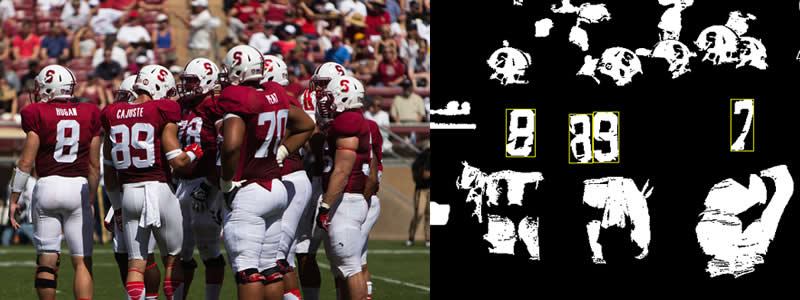
\includegraphics[width=0.8\linewidth]{recognition.jpg}
\caption{Using image processing heuristics to locate digits in an image.}
\end{figure}

%----------------------------------------------------------------------------------------

\end{column} % End of the first column

\begin{column}{\sepwid}\end{column} % Empty spacer column

\begin{column}{\twocolwid} % Begin a column which is two columns wide (column 2)

\begin{columns}[t,totalwidth=\twocolwid] % Split up the two columns wide column

\begin{column}{\onecolwid}\vspace{-.6in} % The first column within column 2 (column 2.1)

%----------------------------------------------------------------------------------------
%	MATERIALS
%----------------------------------------------------------------------------------------

\begin{figure}
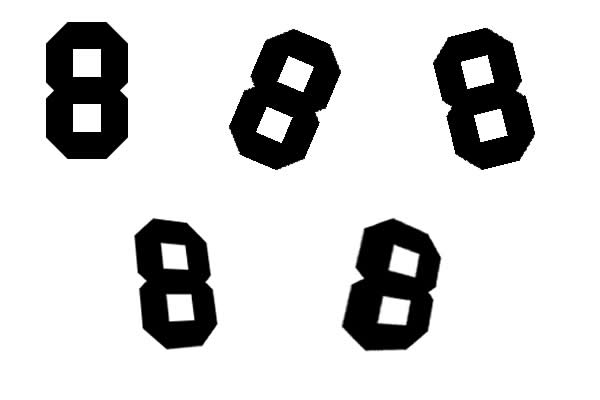
\includegraphics[width=0.8\linewidth]{generated.jpg}
\caption{Synthetic data generated by applying skews and transforms on base images.}
\end{figure}

\begin{block}{Problem Definition}

Our problem is to create a system which takes as input images and outputs a classification as a digit 0-9. This task is similar to handwritten OCR tasks, but adds additional challenges of dimensionality as well as locating the digits in a noisy image in the first place. Given this problem definition, we naturally looked to applying heuristics to image processing in tandem with supervised learning algorithms.

\end{block}

%----------------------------------------------------------------------------------------

\end{column} % End of column 2.1

\begin{column}{\onecolwid}\vspace{-.6in} % The second column within column 2 (column 2.2)

%----------------------------------------------------------------------------------------
%	METHODS
%----------------------------------------------------------------------------------------

\begin{block}{Challenges}

We did not focus on using top-of-line computer vision techniques, and as a result we simplified the problem inputs to images from the Stanford Daily of Stanford football players wearing our home jerseys (red uniforms with white lettering). 

\end{block}

\begin{figure}

\includegraphics[width=0.8\linewidth]{recognized.jpg}
\caption{Results of OCR on digits in Figure 1. With kNN, we achieve 75\% accuracy in this photo.}
\end{figure}

%----------------------------------------------------------------------------------------

\end{column} % End of column 2.2

\end{columns} % End of the split of column 2 - any content after this will now take up 2 columns width

%----------------------------------------------------------------------------------------
%	IMPORTANT RESULT
%----------------------------------------------------------------------------------------

%\begin{alertblock}{Important Result}

%Lorem ipsum dolor \textbf{sit amet}, consectetur adipiscing elit. Sed commodo molestie porta. Sed ultrices scelerisque sapien ac commodo. %Donec ut volutpat elit.

%\end{alertblock} 

%----------------------------------------------------------------------------------------

\begin{columns}[t,totalwidth=\twocolwid] % Split up the two columns wide column again

\begin{column}{\onecolwid} % The first column within column 2 (column 2.1)

%----------------------------------------------------------------------------------------
%	MATHEMATICAL SECTION
%----------------------------------------------------------------------------------------

\begin{block}{K-Nearest Neighbors}

We used the k-nearest neighbors algorithm as a baseline. Our data were the raw images, so the k-nearest neighbors algorithm measured similarity in the 100x100 image space.

\end{block}

\begin{block}{Random Forest}

The random forest classification algorithm makes use of multiple trees from decision tree learning. Each tree is grown over a random subset of the data. An internal node of at ree represents an input feature, and the leaves are labeled with a distribution over the classes. The random forest approach returns the most common classification returned by any of its trees. 

\end{block}

%----------------------------------------------------------------------------------------

\end{column} % End of column 2.1

\begin{column}{\onecolwid} % The second column within column 2 (column 2.2)

%----------------------------------------------------------------------------------------
%	RESULTS
%----------------------------------------------------------------------------------------

\begin{block}{Support Vector Machines}

Our main design decisions were made in choosing the feature representation and the kernel. For the feature, we used Histogram of Oriented Gradients (HoG), which has been known to work well in digit recognition. We use the Sobel operator to compute the gradient of the image. We divide the image into four bins and compute the histogram. We experimented with different bin sizes, but since our images were already only 100x100 pixels, four bins seemed to work better than 16, etc. We are currently using the radial basis function $K(x_i, x_j) = \mbox{exp }(-\gamma \|x_i - x_j\|^2)$ for the kernel. We have experimented with polynomial kernels, but limited testing data prevents us from arguing strongly for one kernel over the other.

\end{block}

%----------------------------------------------------------------------------------------

\end{column} % End of column 2.2

\end{columns} % End of the split of column 2

\end{column} % End of the second column

\begin{column}{\sepwid}\end{column} % Empty spacer column

\begin{column}{\onecolwid} % The third column

%----------------------------------------------------------------------------------------
%	CONCLUSION
%----------------------------------------------------------------------------------------

\begin{block}{Results}

We train our classifiers on 69 distinct transformations of each digit, and test on $n=30$ samples. We are able to obtain a 76.78\% accuracy using kNN on raw pixel data, a 50.00\% accuracy using SVMs with the HoG feature, and a 33.33\% accuracy with random forests and the HoG feature.

\end{block}

%----------------------------------------------------------------------------------------
%	ADDITIONAL INFORMATION
%----------------------------------------------------------------------------------------

\begin{block}{Analysis}

We were surprised at how simple heuristics can go a long way in addressing OCR issues. kNN represented a rather naive way of looking at the problem space, but also turned out to be the most effective. In additon, we found that normalizing the test data to be of a consistent size and position had an enormous impact on the classifiers and their ability to perform. 

\end{block}

\begin{block}{Conclusion}

We find that digits can be reliably isolated from an arbitrary image through heuristic-based image processing. We also find that synthetic training data generated from a base font and skewed across a variety of transforms is appropriate as a training corpus for this jersey ORC task. When these two processes are chained together, we are able to identify players that are represented in a photo. 

\end{block}

%----------------------------------------------------------------------------------------
%	REFERENCES
%----------------------------------------------------------------------------------------

\begin{block}{References}

% \nocite{*} % Insert publications even if they are not cited in the poster
% \small{\bibliographystyle{unsrt}
% \bibliography{sample}\vspace{0.75in}}
\small{\begin{enumerate}
\item Bradski, G. OpenCV. Dr. Dobb's Journal of Software Tools, 2000.
\item Saric, M., Dujmic, H., Papic, V., Rozic, N. Player number localization and recognition in soccer video using HSV color space and internal contours.
\end{enumerate}}

\end{block}

% %----------------------------------------------------------------------------------------
% %	ACKNOWLEDGEMENTS
% %----------------------------------------------------------------------------------------

% \setbeamercolor{block title}{fg=red,bg=white} % Change the block title color

% \begin{block}{Acknowledgements}

% \small{\rmfamily{Nam mollis tristique neque eu luctus. Suspendisse rutrum congue nisi sed convallis. Aenean id neque dolor. Pellentesque habitant morbi tristique senectus et netus et malesuada fames ac turpis egestas.}} \\

% \end{block}

% %----------------------------------------------------------------------------------------
% %	CONTACT INFORMATION
% %----------------------------------------------------------------------------------------

% \setbeamercolor{block alerted title}{fg=black,bg=norange} % Change the alert block title colors
% \setbeamercolor{block alerted body}{fg=black,bg=white} % Change the alert block body colors

% \begin{alertblock}{Contact Information}

% \begin{itemize}
% \item Web: \href{http://www.university.edu/smithlab}{http://www.university.edu/smithlab}
% \item Email: \href{mailto:john@smith.com}{john@smith.com}
% \item Phone: +1 (000) 111 1111
% \end{itemize}

% \end{alertblock}

% \begin{center}
% \begin{tabular}{ccc}
% 
\includegraphics[width=0.4\linewidth]{logo.png} & \hfill & 
\includegraphics[width=0.4\linewidth]{logo.png}
% \end{tabular}
% \end{center}

%----------------------------------------------------------------------------------------

\end{column} % End of the third column

\end{columns} % End of all the columns in the poster

\end{frame} % End of the enclosing frame

\end{document}
